\chapter{Configure access and security for instances}\label{cha:conf-access-secur}
The security and accessibility of your cloud resources is governed by
a few different aspects, which we discuss more detail in the following
sections:
\begin{itemize}
\item Instances must connect to the project's \_vm network in order to
  get external internet access (see section \ref{sec:_vm-_nfs-networks}).
\item Each cloud project can use one floating IP, a public IP address
  which you'll need to link to the resources you want to access. Optionally,
  if the project has requested access to VSC network it will receive also
  three VSC floating IPs (see section \ref{sec:floating-ip}).
\item By default, the UGent firewall blocks most IP addresses and
  ports.  Only the port range 50000-60000 for the public floating IP
  addresses is open by default.
  Contact \cloudinfo if you need to access other ports from the
  outside world.
\item The OpenStack environment has its own internal firewalls, which
  block most ports of your instances by default.  If you want to
  access specific ports of your instances, you must create ``Security
  Groups'' which allow access to those ports (see section
  \ref{sec:security-groups}).
\item You can use one or more SSH keys from your VSC account to access
  your instances (see section \ref{sec:ssh-key-pairs}).
\end{itemize}
For other access methods, or SSH authentication for a wider set of
users, you'll need to set up some form of identity management
yourself.  This system administration task is beyond the scope of our
tutorial.

\section{The \_vm, \_vsc and \_nfs networks}\label{sec:_vm-_nfs-networks}
Each project in the VSC cloud has its own network
\texttt{\emph{<projectname>}\_vm} and --- if the project uses shares
and/or vsc networks --- \texttt{\emph{<projectname>}\_nfs} and 
\texttt{\emph{<projectname>}\_vsc} respectively. Each is a subnet of 254
addresses, with an ip range 10.10.$x$.0/24, where $x$ is a number that
depends on the project and network.  To see the subnets for your
project's networks, open the Network tab, and select Networks.

Instances should use the \_vm network for communication, and the \_nfs
network if they need access to shared file systems (see chapter
\ref{cha:shared-file-systems}). On the other hand \_vsc network is used to
connect to or provide VSC services via VSC network and floating IPs.
When an instance is created in
\gls{OpenStack} and connected to the \_vm, \_nfs or \_vsc networks, it is
automatically assigned a fixed IP address in that network. This IP
address is permanently associated with the instance until the instance
is terminated.

\section{Floating IP addresses}\label{sec:floating-ip}
The \_vm, \_nfs and \_vsc networks can only be reached from within the
OpenStack environment.  If you need to access an instance from the
outside, you need to use one of your project's floating IP addresses,
which are public IP addresses (193.190.80.0/25 IPs for \_vm network) or
VSC IP addresses (172.24.48.0/20 IPs for \_vsc network).
Unlike fixed IP addresses, floating IP addresses can have their associations
modified at any time, regardless of the state of the instances involved.

\strong{Note:} Do not release the floating IPs assigned to your project.
The floating IPs are fixed to the project and it is not possible, as regular user,
to re-allocate floating IPs.
Please contact to VSC Tier1 Cloud support \cloudinfo if you have released
your project's floating IPs by mistake.

This section explains how to make your instance accessible via a
public IP address by two different methods. The preferred method for \_vm
network is to use port forwarding to access multiple instances using the
same public IP address, but you can also use a ``floating IP association''
for quick tests or \_vsc network.

\subsection*{Floating ip port forwarding}
OpenStack's networking API, called Neutron, makes it possible to
forward different ports of the same floating ip to arbitrary ports in
one of OpenStack's virtual networks.  This is the recommended way to
use floating ip's in the VSC cloud.  For the floating IP's available
in the VSC Cloud, the high port range 50000-60000 is open to the
outside world, so it is most convenient to work with ports from this
range.  Contact \cloudinfo if you need public access to another port
for a specific ip address.

You'll need to forward a separate port for every service you wish to
reach.  For example, if you want to access an instance using SSH,
you'll need to create a port forwarding rule from a selected port of
the floating IP, to the port in the \_vm network where your instance's
SSH server is listening (typically port 22).

You can quickly set up such forwarding rules using
\lstinline{neutron_port_forward}, a command line tool available on the
UGent login node, \lstinline{login.hpc.ugent.be}.  In order to use it,
you must create an application credential for the role ``User'', and
save it as an openrc file (see section \ref{sec:appl-cred} on page
\pageref{sec:appl-cred}).  Transfer the openrc file to your VSC
storage space, so \lstinline{neutron_port_forward} can read it.  To
set up new port forwarding rules, run the script providing the path to
the openrc file as an argument to the \lstinline{-o} option, and a
file describing your port forwarding configuration as argument to the
\lstinline{-m} option:

\begin{prompt}
  % \shellcmd{neutron\_port\_forward -o <openrc file.> -m <ini-file>}
\end{prompt}

The following is an example configuration file:
\begin{code}{}
[DEFAULT]
floatingip=193.190.85.40
network=_vm

[classa]
pattern=classa-(\d+)
22=52000:100:22
5900=55900

[classb]
pattern=classb-(\d+)
80=52080
\end{code}

Here we define defaults for the floating ip and target network, and
two classes.  Instances are assigned to a class if their name matches
the regular expression given in \lstinline{pattern}.  The value of
\lstinline{pattern} must be a valid Python regular expression, and the
first capturing group (if any) must match an integer.

Port forwarding rules are given in the form
\lstinline{target=source(:multiplier:offset)}.  This will set up a
forwarding rule from the floating IP port

$$ (\mathrm{source} + \mathrm{multiplier} * i + \mathrm{offset}) \rightarrow \mathrm{target}\, ,$$

where $i$ is the integer matched by the first capturing group, and
``target'' is a port of the fixed IP for the instance in the chosen
network, in this case the \_vm network.  ``multiplier'' and ``offset''
are optional and default to 1 and 0 respectively.  In our example,
this results in the following set of port forwarding rules for
the public IP address 193.190.85.40:

\begin{center}
  \texttt{
\begin{tabular}{l>{$\rightarrow$\ \ }l}
  52122 & classa-1:22\\
  52222 & classa-2:22\\
  \ldots\\
  55901 & classa-1:5900\\
  55902 & classa-2:5900\\
  \ldots\\
  52081 & classb-1:80\\
  52082 & classb-2:80\\
  \ldots
\end{tabular}
}
\end{center}

You can also see an overview of existing port forwarding rules for the
ip addresses in your configuration file using
\lstinline{neutron_port_forward --show}.  Each rule has an internal
id, which you can see if you combine the options \lstinline{--show}
and \lstinline{--id} as follows:

\begin{prompt}
  % \shellcmd{neutron\_port\_forward -o <openrc file.> -m <ini-file> ---show ---id}
\end{prompt}

To remove port forwarding rules, use the option
\lstinline{--remove=<list of id's>} with a comma-separated list of the
id's of the rules you want to remove.  Rules are removed automatically
if the target instance is deleted.

\lstinline{neutron_port_forward} provides a few more options and
advanced features, run the command with the \lstinline{--help} option
for more information.

\subsection*{Associate a floating ip}
A floating IP address can also be associated to an instance, just like
the fixed IP addresses.  Because this approach uses one of the few
available floating ip addresses for every instance you want to connect
to, you should only use it for testing purposes with \_vm network or
with \_vsc network.

\strong{Note:} If you want to use a floating ip for port forwarding as
in the previous section, it cannot be associated to an instance at the
same time.

Use the following procedure to associate that address with a specific
instance.

\begin{enumerate}
\item Open the Network tab.
\item Click the Floating IPs tab, which shows the floating IP
  addresses allocated to your project.
\item In the Floating IPs list, click Associate next to the address you want.
\item In the Manage Floating IP Associations dialog box, choose the
  following options:

  \begin{description}
  \item[IP Address] This field is filled automatically.
  \item[Port to be associated] Select a port from the list.  The list shows all the instances with their fixed IP addresses.
  \end{description}
\item Click Associate.
\end{enumerate}

Another way to associate a floating IP is after the user has already launched an instance which appears in the list of running instances in the Project-->Compute-->Instances tab:

\begin{enumerate}
\item Expand the drop-down menu on right next to the instance
\item Select Associate Floating IP
\begin{center}
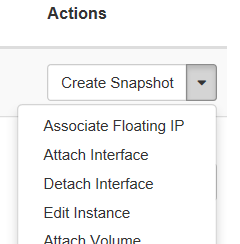
\includegraphics[scale=0.7]{img/associate_IP_1.png}
\end{center}
\item A pop-up window will appear and under IP Address select from the
  drop-down menu an IP address from the available pool.
\begin{center}
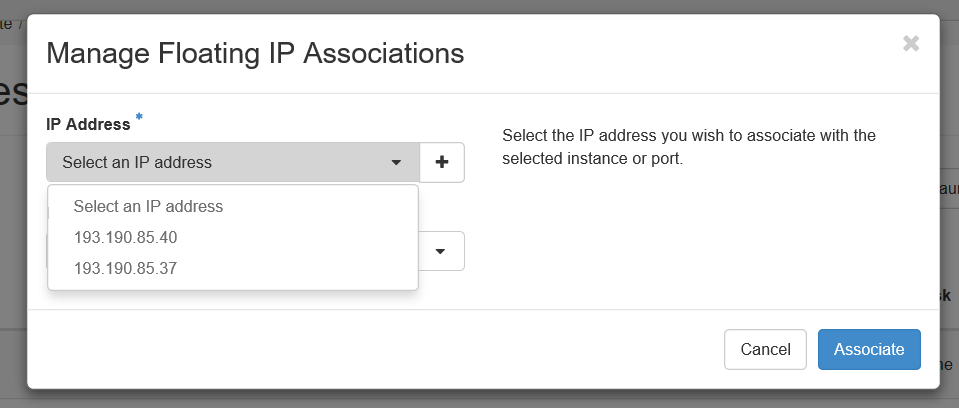
\includegraphics[scale=0.5]{img/associate_IP_2.png}
\end{center}
\item Click Associate
\end{enumerate}

If the IP has been successfully associated in the upper right corner of the browser screen will appear a green confirmation. If not successful a red notification will pop up that something went wrong.

\strong{Note:} To disassociate an IP address from an instance, click
the Disassociate button in the Actions column.

% TODO: remove this warning once we've removed the "Release Floating
% IP" buttons from the dashboard.
\strong{Warning:} \emph{Do not} use the Release Floating IP option in
the Actions column or on the overview page.  This will remove the
floating IP from the pool assigned to your project, something which
you, as a regular user, cannot undo.  If you've accidentally released
a floating IP, contact \cloudinfo to have it restored.

\section{Security Groups}\label{sec:security-groups}
OpenStack security groups are sets of IP filter rules that define
networking access.  You can then assign one or more security groups to
your instances.

In the VSC cloud, each project contains a default security group,
which allows you to ping instances and connect using SSH on the
default port 22.  If you want to access other ports on your instances,
create new security groups with the appropriate rules and assign them
to the instances.

\section{SSH key pairs}\label{sec:ssh-key-pairs}
When an instance is launched, OpenStack can automatically install a
public SSH key on it, so as to give anyone with the corresponding
private key admin access.  For this ``key pair injection\footnote{The
  OpenStack documentation and interfaces consistently refer to ``SSH
  pairs'', but of course only the public key of each pair is stored in
  the OpenStack environment, while the private key should be kept
  secure by the owner.}'' to work, the image that the instance is
based on must contain the \textbf{cloud-init} package, or have in
place another mechanism in place that will interact with the OpenStack
metadata server to install the appropriate key.  For general
instructions on SSH keys, we refer to chapter 2 of our
\href{https://hpcugent.github.io/vsc\_user\_docs}{introduction to
  HPC}.

If you have generated a key pair with an external tool, you can import
it into OpenStack. The key pair can be used for multiple instances
that belong to a project. For more information, see section
\ref{import-a-key-pair}.

\strong{Note:} The public keys from your VSC account are automatically
available in your VSC Cloud projects, so you can immediately inject
one of your existing into your instances.  Of course, you can also
import new keys into OpenStack, which are not coupled to your VSC
account.  If you want to give other parties SSH access to VM's, you
must manage the keys using some other method.  \strong{Never} upload
SSH keys for other users to your VSC account.

\strong{Note:} Every OpenStack user account has its own collection of
SSH keys for every project.  To share a public key between multiple
users of the same project, each user needs to import it in the
OpenStack project.

\subsection*{Add a key pair}\label{add-a-key-pair}
\begin{enumerate}
\item Open the Compute tab.
\item Click the Key Pairs tab, which shows the key pairs that are
  available for this project.
\item Click Create Key Pair.
\item In the Create Key Pair dialog box, enter a name for your key
  pair, and click Create Key Pair.
\item Respond to the prompt to download the key pair.
\item Save the \textbf{*.pem} file locally.
\item To change its permissions so that only you can read and write to
  the file, run the following command:

  \begin{prompt}
      %\shellcmd{chmod 0600 yourPrivateKey.pem}
  \end{prompt}

  \strong{Note:} If you are using the \gls{OpenStack Dashboard} from a
  Windows computer, use PuTTYgen to load the \textbf{*.pem} file and
  convert and save it as \textbf{*.ppk}.  For more information see the
  \href{https://winscp.net/eng/docs/ui_puttygen}{\emph{WinSCP web page
      for PuTTYgen}}, and chapter 2 of the
  \href{https://hpcugent.github.io/vsc\_user\_docs}{introduction to
    HPC at VSC}.

\item To make the key pair known to SSH, run the \textbf{ssh-add}
  command.

  \begin{prompt}
    %\shellcmd{ssh-add yourPrivateKey.pem}
  \end{prompt}
\end{enumerate}

\subsection*{Import a key pair}\label{import-a-key-pair}
\begin{enumerate}
\item Open the Compute tab.
\item Click the Key Pairs tab, which shows the key pairs that are
  available for this project.
\item Click Import Key Pair.
\item In the Import Key Pair dialog box, enter the name of your key
  pair, copy the public key into the Public Key box, and then click
  Import Key Pair.
\end{enumerate}

The Compute database registers the public key of the key pair.

The \gls{OpenStack Dashboard} lists the key pair on the Key Pairs tab.

%%% Local Variables:
%%% mode: latex
%%% TeX-master: "intro-Cloud"
%%% End:
